\chapter{Feature Extraction}

总结文章:\href{https://zhuanlan.zhihu.com/p/35724768}{Object Detection总结 Two Stage}

总结文章:\href{https://zhuanlan.zhihu.com/p/35731743}{Object Detection总结 One Stage}

\section{Selective Search}

\subsection{Efficient Graph-Based Image Segmentation}

Selective Search基于文章\cite{Felzenszwalb2004}中基于图分割的图像分割技术。

论文\cite{Felzenszwalb2004}提出的是一种基于贪心选择的图像分割算法,论文中把图像中的每个像素表示图上的一个节点,每一条连接节点的无向边都具有一个权重(weights),以衡量其连接的两个节点之间的不相似度,这篇论文的创新点在于该算法能够根据相邻区域在特征值上变化速度的大小动态调整分割阈值。这个特征值就是类间距离和类内距离,如果类间距离大于类内距离就认为是两个区域。定义类内距离为对应区域的最小生成树(因为把图像看做一个连接图,所以每个区域可以用最小生成树来表示)中权重最大的边的权重值,类间距离定义为两个区域内相邻点的最小权重边,如果两个区域没有相邻边则取无穷大。但是这样其实还是有问题,比如一个类中只有一个点的时候,它的类内距离为0,这样就没法搞了(每个点都变成了一类,此时类内距离变为0),所以作者又引入了一个阈值函数,用来表示两个区域的区域的类间距离至少要比类内距离大多少才能认为是两个区域。

判断两个点$C_1$与$C_2$是否属于同一类的判定:
\begin{displaymath}
D(C_1, C_2) = 
\begin{cases}
true & \text{if } Dif(C_1, C_2) > M Int(C_1, C_2)\\
false & \text{otherwise}
\end{cases}
\end{displaymath}
其中,$MInt(C_1, C_2)$为判断类间间距$Dif$的阈值,由类内间距计算得到:
\begin{displaymath}
M Int(C_1, C_2) = \min (Int(C_1) + \tau (C_1), Int(C_2) + \tau (C_2) )
\end{displaymath}
其中,$\tau$即为控制当类间的最短距离。一般取为$C$的负相关函数,$k$为常数:
\[
\tau(C) = k / |C|
\]
当$k$的取值大时,类间距要求大,所以分割后的区域面积也会较大,否则区域面积较小。

具体的分割过程,可以参考文章\cite{Felzenszwalb2004}的\textbf{Algorithm 1}。

\subsection{Selective Search}
主要参考文献:\cite{Uijlings2013}

接下来介绍Selective Search算法,该算法利用\cite{Felzenszwalb2004}的图分割算法获得的分割区域结果,再一次根据一些搜索策略(相似度)做了一个聚类。也是和上面的思路一致,首先根据获得的区域,算出每个区域和其他区域的相似度,不相邻的和自身与自身的相似度都设置为0,得到一个N*N的矩阵,然后将相似度最大的合并,再次计算相似度矩阵(这里是增量更新,只需要计算新生成的区域和其他区域的相似度就可以了),这样合并一次较少一个区域,对于N个区域需要执行N-1次合并,最终得到一个区域。对于相似度的度量,作者主要选取了颜色和区域两大块,颜色作者比较了8种模型,最终选择了HSV,区域主要考量大小、纹理和吻合度(相交包含关系)这三个因素。





\section{Region CNN}

\subsection{概述}

\begin{figure}[!htbp] 
\centering
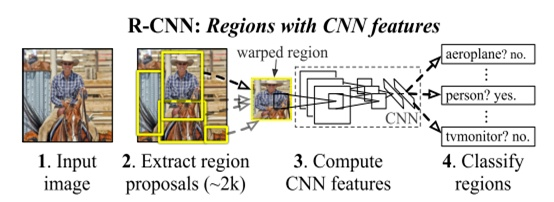
\includegraphics[width=0.85\textwidth]{FeatureExtraction/RCNN0.jpg}
\caption{RCNN整体思想 }
\label{RCNN0}
\end{figure}

这里的 Extract region proposals 是基于Selective Search实现的,然后将这些候选框输入到CNN进行特征提取,最后利用SVM对提取的特征进行分类。


\subsubsection{Boundingbox 回归}




\section{SPP Net}

参考文献:\cite{he2014spatial}

在这之前的网络都要求输入图像数据的大小是固定的,而本文提出了Spatial pyramid pooling, 可以允许输入图像是任意大小,并且都会生成一个固定大小的表示。

此外,Pyramid pooling用于目标检测时,可以提高RCNN的速度,因为只需要对整幅图像提取一次特征,然后在Pooling层进行获取sub-images。

\subsection{背景与相关工作}

固定输入图像的大小,不利于识别在不同Scale下的目标。

那么为什么会有这种限制呢?传统的CNN结构可以认为由Convolution lyaers和Fully connected layers两部分组成,前者对输入尺寸没有要求,且可以输出任意的尺寸;但是后者的输入对尺寸有要求,所以限制了输入图像的尺寸。训练的时候也可以使用不同尺寸的
图像进行训练。

改进的Spatial Pyramid Pooling在网络结构中的位置:
\begin{figure}[!hbtp]
\centering
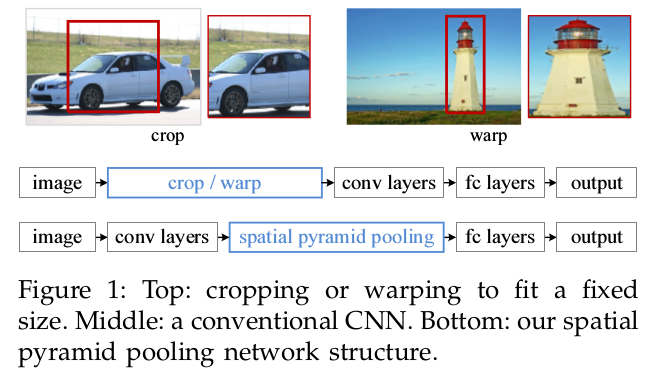
\includegraphics[width=0.75\textwidth]{FeatureExtraction/SPPNet0.png}
\caption{Pyramid Pooling在网络结构中的示意图,与传统CNN结构的比较}
\label{SPPNet0}
\end{figure}

即在Convolution部分的最后一层之后,加入了Pyramid Layer, 可以认为是一种Information Aggregation。

本文在Feature Map上对识别器进行训练与测试。

基于最近新提出的一个Fast proposal method of EdgeBoxes。

\subsection{网络结构}

\subsubsection{Fisher Kernel}

参考文献:\href{https://en.wikipedia.org/wiki/Fisher_kernel}{Fisher Kernel Wikipedia}

目的是,通过对两个object进行一系列的Measurements和一个Statistical model, 得到两个Object的相似性。

在分类中,可以通过最小化New object与each known number of the given class之间的Fisher Kernel distance来实现分类。

Fisher Kernel 借鉴了生成模型和判别模型:
\begin{itemize}
\item 生成模型可以处理任意长的数据
\item 判别模型可以have flexible criteria和得到更好的结果
\end{itemize}

Fisher Kernel基于Fisher Score来实现:
\begin{displaymath}
U_X = \nabla_\theta \log P(X | \theta)
\end{displaymath}

其中,$\theta$ 是模型参数,$\log P(X|\theta)$是对数似然。

然后Fisher Kernel如下:
\begin{displaymath}
K(X_i, X_j) = U_{X_i}^TI^{-1}U_{X_j}
\end{displaymath}

其中, $I$是Fisher Information matrix,比较复杂,查Wikipedia吧。

一种应用是:用在图像分类和Retrieval中,由于Bag of visual words模型 suffer from sparsity 和 high dimensionality。而Fisher Kernel可以产生稠密、Compact的Representation。

\subsubsection{Convolutional Layers and Feature Maps}

在强调一下,对输入图像固定尺寸这一限制来自于全连接层的输入要求。基于传统的特征表示的,会再利用其他技术进行表示的处理,如上文提到的Fisher Kernel等。

\subsubsection{The Spatial Pyramid Pooling Layer}

相比于传统的基于BoW的模型,Spatial pyramid pooling还可以保留空间信息 by pooling in local spatial bins, These spatial bins have sizes proportional to the image size, so the number of bins is fixed regardless of the image size.(这句话有错误吧,先说这些Spatial bins与输入图像大小成正比,但又说the number of bins是固定的,与图像尺寸无关。???)

图表示了提出的Pyramid Pooling Layer的示意图。在每一个Spatial bin, 作者对每一个filter 的 response进行Pool(MaxPooling)。 而输出是$kM$, 其中,$k$是filter的数目,$M$是the number of bins? 这里的bin是指Pooling后的结果么?然后结果被输入到Fully connected层。

\begin{figure}[!hbtp]
\centering
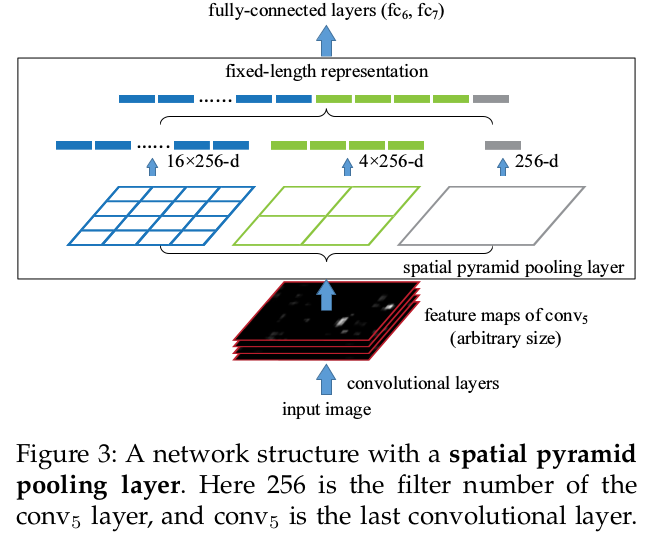
\includegraphics[width=0.75\textwidth]{FeatureExtraction/SPPNet1.png}
\caption{Pyramid Pooling的计算过程示意图}
\label{SPPNet1}
\end{figure}

作者证明,在深度网络中,多尺度对提高精度同样重要。

作者认为:The global pooling operation corresponds to the traditional BoW method.?

\subsubsection{Training}

在这部分,作者貌似提到了Pyramid Pooling是怎么进行的。得到最后一层的$a \times a$ 大小的 Feature Map进行Pooling操作,操作时,Sliding window Pooling 的 window size 是 $win = \lceil a / n \rceil$, 然后Pooling的stride是$\lfloor a / n \rfloor$。

基于 cuda-convnet 和 caffe实现。

\subsection{Object Detection Experiments}

在分类的试验中,实验结果表明,Multi-level Pooling提高精度, Multi-size也提高精度, Fully-image representation 提高精度、

Model Combination是提高CNN-based 分类器精度的一种重要手段。实验表明,这种提升貌似来自于Convolutional layer。如果组合两个具有一样结构的Conv,那么效果貌似并没有提升。

这个细节还是有必要说一下。

RCNN的工作流程是:首先用Selective search在输入图像上得到候选框,然后进行在每一个候选框输入到CNN进行特征提取,提取的特征送入SVM进行分类。

注意,因为与之前的方法相比,在目标识别中,本分的方法只对整幅图像进行一次卷积,然后在Feature Map进行选框操作(Candidate window of feature maps)。那么这个在Feature Map中的候选框是怎么来的呢?

看文章附件的意思:

首先在输入图像中生成候选框,可以用相同的Selective方法等, 在Image Domain生成一系列的候选框,然后把这个候选框的位置映射到Feature Map中,得到其在Feature map中的Corner point。由于在得到Feature Map的过程中涉及很多的下采样过程,所以,在映射的过程中需要注意映射的准确性。本文用到的映射公式如下:
\begin{displaymath}
\begin{gathered}
x' = \lfloor x/S  \rfloor + 1 \qquad  (left top corner)\\
x' = \lfloor x/S \rfloor - 1 \qquad (right bottom corner)
\end{gathered}
\end{displaymath}

其中$S$是当前层的Stride。上述过程的前提是,Padding为$\lfloor p/2 \rfloor$。$p$为Pooling的size。

\subsection{Conclusion}

SPP is a flexible solution for handling different scales, sizes, and aspect ratios. The resulting SPP-net shows outstanding accuracy in classification/detection tasks and greatly accelerates DNN-based detection.

还有就是,一些经典的视觉算法在深度学习中,同样可以发挥重要的作用!

\section{Fast RCNN}

参考文献:

[2] \href{https://zhuanlan.zhihu.com/p/27640199}{详解ROI-Pooling层的实现-知乎}

\subsection{ROI-Pooling层的实现-知乎}

Fast-RCNN的大体步骤:
\begin{itemize}
\item 输入: images的shape是(N, W, H, C)这是Tensorflow的输入。Rois的shape是(nums\_rois, 4)这里注意了,ROI也是输入的参数,那么这些ROI怎么来的呢,可能是Selective Search的结果。

\item VGG网络对输入的Image部分提取特征,走到最后一层卷积层

\item 最后一个卷积层的输出作为OI Pooling层的输入

\item ROI Pooling的输出在做分类和回归
\end{itemize}

\subsubsection{ROI Pooling层}

输入Shape: (N, W/16, H/16, channels), 因为是使用VGG16实现,经过4次2*2的Max Pooling,所以降维16倍,这里的Pooling默认Strides为2.

输出Shape: (num\_rois, expected\_H, expected\_W, channels), 论文中提到如果使用VGG16, 则输出是W= H = 7。

由于输入的图像下采样了16倍,所以输入的ROI也会缩小16倍,包括索引、长宽等。





 
\subsection{RoI Pooling}




\section{Faster RCNN}

\section{R FCN}


\section{FPN}


\section{Mask RCNN}


\section{YOLO}


\section{YOLO v2}


\section{YOLO v3}


\section{SSD}


\section{DSSD}


\section{Retina Net (Focal Loss)}

\section{Feature Pyramid Network}

在处理高层但分辨率小的特征图与底层但分辨率高的特征图的时候,使用Nearest neighbor interpolation的方法进行Upsample。

\subsection{Nearest Neighbor Interpolation}

参考:\href{https://blog.csdn.net/linqianbi/article/details/78593724}{最近邻插值}

这是一种简单的插值算法:不需要计算,在待求象素的四邻象素中,将距离待求象素最近的邻象素灰度赋给待求象素

设i+u, j+v(i, j为正整数, u, v为大于零小于1的小数,下同)为待求象素坐标,则待求象素灰度的值 f(i+u, j+v)

如果(i+u, j+v)落在A区,即u<0.5, v<0.5,则将左上角象素的灰度值赋给待求象素,同理,落在B区则赋予右上角的象素灰度值,落在C区则赋予左下角象素的灰度值,落在D区则赋予右下角象素的灰度值。
最邻近元法计算量较小,但可能会造成插值生成的图像灰度上的不连续,在灰度变化的地方可能出现明显的锯齿状。

\section{ResNet}

最需要明确的是:ResNet现在基本上作为各种视觉算法的Backbone了!!!要知道Backbone的牛逼。

然后需要注意以下两点:再由ResNet18 到ResNet50的时候是把基本block扩展为bottleneck,这个bottleneck就是输出Channel先变小在变大!第二点是:Identity 和 Non-Identity两条路径的结果是通过相加实现的,分辨率不同的时候会先通过Maxpooling降维!






